\section{Interpolation schemes}

\label{sec_lptinterpolation}

For updating the particle properties (velocity, position, etc.), local properties of the continuous phase  is interpolated.
This function is implemented in lagrangian\_forces.cpp.

%-----------------%
%                 %
%  Interpolation  %
%                 %
%-----------------%
\begin{figure}[ht]
  \centering
  \setlength{\unitlength}{ 1mm}
  \begin{picture}( 250, 50)( 0, 0)
    \thickbox{ 250}{ 50}
    \put( 40, 0){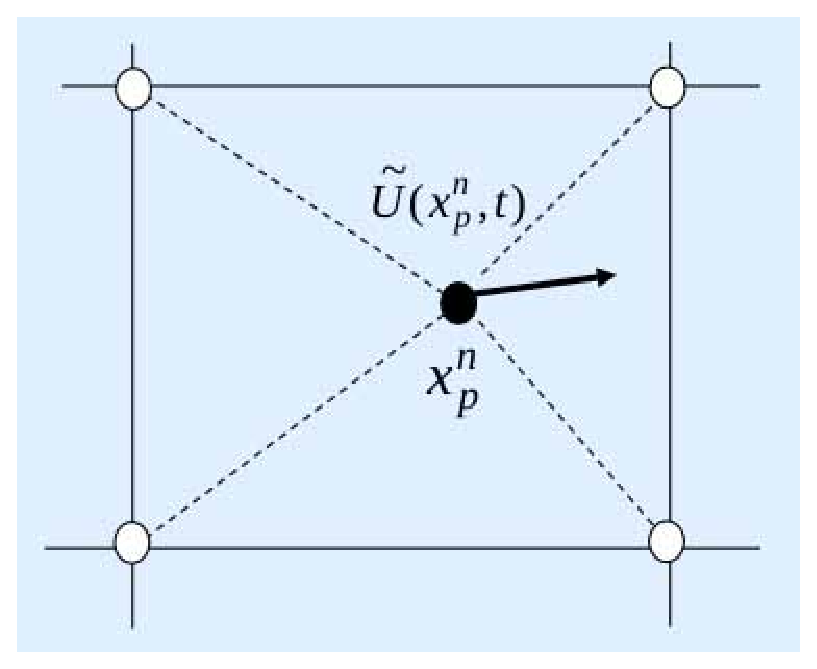
\includegraphics[scale=0.50]{Figures/10-LPT/10-02-interpolation.eps}}
  \end{picture}
  \caption{Basic idea about interpolating the continuous properties on particle location.}
  \label{fig_interpolation}
\end{figure}

Four different kinds of interpolation schemes are implemented for Lagrangian particle tracking in {\psiboil}, defined by the mark number.

\begin{itemize}
  \item {1,  dispersed boxing interpolation}, 
  \item {2,  local one-cell approach}, 
  \item {3,  2nd order Lagrange interpolation\footnote{\tt Dr. A. Dehbi, Paul Scherrer Institut, Lagrangian Methods for Dispersed Particle Flows: Lecture 2: Particle tracking in Laminar Flows, ETHZ, Zurich, 27.03.2017}}, 
  \item {4,  linear interpolation}.
\end{itemize}

\subsection{Equations of 1D Lagrange interpolation}

The first, the second and the n-th order 1D Lagrange interpolation formulas\footnote{\tt www-classes.usc.edu/engr/ce/108/lagrange.pdf} share the same form:

%
\be
    f(x)
    = {f_0}{\delta_0}(x) + {f_1}{\delta_1}(x) + ... + {f_i}{\delta_i}(x) + ... + {f_n}{\delta_n}(x)
    \;\;\;\;
    (i=0,...,n)
  \label{eq_1DnthLagrangeinterpolation}
\ee
%

in which, ${\delta_i}(x)$ can be written as

%
\be
    {\delta_i}(x)
    = \frac{\prod_{i=0, i \neq j}^{n} (x-x_i)}
           {\prod_{i=0, i \neq j}^{n} (x_j-x_i)}
  \label{eq_1DnthLagrangeninterpolationdelta}
\ee
%

Each term of ${\delta_i}(x)$ has the required properties such that:

\begin{itemize}
  \item {${\delta_i}(x_j)$=0, when $i \neq j$}
  \item {${\delta_i}(x_j)$=1}
\end{itemize}

The above property ensure $f(x_i)=f_i$ and none of the other samples values $f_i, i \neq\ j$ participate.


\subsection{Equations of 3D 2nd order Lagrange interpolation}

Setting the interpolation scheme mark is 3, thus the 3D independent 2nd order Lagrange interpolation is adopted.
The related equations are:

%
\be
    f(\underline{x})
    \approx p_m(x)
    =  {\sum_{i=0}^m} {\sum_{j=0}^m} {\sum_{k=0}^m} f(i,j,k) L_i(x_1) L_j(x_2) L_k(x_3)
    \;\;\;\;
    \underline{x}=(x_1,x_2,x_3)
  \label{eq_3D2ndorderLagrangeinterpolation}
\ee
%

%
\be
    L_i(x_1)
    = {\prod_{n=0, n \neq i}^m} \frac{x_1-x_{1,n}}{x_{1,i}-x_{1,n}}
  \label{eq_3D2ndorderLagrangeinterpolationLi}
\ee
%

%
\be
    L_j(x_2)
    = {\prod_{n=0, n \neq j}^m} \frac{x_2-x_{2,n}}{x_{2,j}-x_{2,n}}
  \label{eq_3D2ndorderLagrangeinterpolationLj}
\ee
%

%
\be
    L_k(x_3)
    = {\prod_{n=0, n \neq k}^m} \frac{x_3-x_{3,n}}{x_{3,k}-x_{3,n}}
  \label{eq_3D2ndorderLagrangeinterpolationLk}
\ee
%
